\documentclass{article}
\usepackage[utf8]{inputenc}
\usepackage[T1]{fontenc}
\usepackage{booktabs}
\usepackage{graphicx}
\usepackage[margin=1in]{geometry}

\title{Ablação RGAT vs.\ T5 puro no Spider}
\author{}
\date{}

\begin{document}
\maketitle

\section{Introdução}

Esta nota documenta um experimento de ablação complementar ao estudo principal
no ScienceBenchmark: treinar variantes \emph{sem} RGAT (t5-small e t5-base
padrão, sem nenhuma estrutura de grafo) diretamente no Spider -- o mesmo
benchmark e orçamento de treino (5 épocas) usados para produzir o checkpoint
de referência com RGAT (t5-base + RGAT, 41,9\% \emph{exact match} / 44,8\%
\emph{execution accuracy} no dev set do Spider, 1034 exemplos). O objetivo é
isolar se a vantagem do RGAT observada na literatura se sustenta quando
comparada a um T5 padrão treinado com o mesmo orçamento, no próprio terreno de
origem da arquitetura (esquemas pequenos e homogêneos do Spider).

\section{Tabela de métricas}

\begin{table}[h]
\centering
\caption{Todas as métricas de avaliação, dev set completo do Spider (1034 exemplos).}
\label{tab:spider-ablation}
\begin{tabular}{lrrrrr}
\toprule
\textbf{Configuração} & \textbf{exact match} & \textbf{exec} & \textbf{eval\_loss} & \textbf{train\_loss} & \textbf{tempo de treino} \\
\midrule
t5-base + RGAT (referência) & \textbf{41,9\%} & \textbf{44,8\%} & -- & -- & -- \\
t5-small \textbf{sem} RGAT (5 épocas) & 13,93\% & 16,25\% & 0,5965 & 1,2751 & 1h42min \\
t5-base \textbf{sem} RGAT (5 épocas) & 41,10\% & 43,81\% & 0,2526 & 0,5793 & 3h12min \\
\bottomrule
\end{tabular}

\vspace{0.4em}
{\footnotesize A linha de referência (t5-base + RGAT) reflete o checkpoint já
publicado no estudo principal (\texttt{docs/sciencebenchmark-eval-results.tex}),
treinado com a mesma metodologia (5 épocas, mesmo split de treino/dev) --
\texttt{eval\_loss}/\texttt{train\_loss}/tempo de treino não foram re-extraídos
para esta nota. As demais linhas são de treinos novos, executados
especificamente para esta ablação.}
\end{table}

\section{Achado principal}

O resultado é notável: o \textbf{t5-base sem RGAT praticamente empata com o
checkpoint RGAT de referência} (41,10\% vs.\ 41,9\% exact match; 43,81\% vs.\
44,8\% exec -- uma diferença de menos de 1 ponto percentual em ambas as
métricas). Isso contrasta com a intuição de que o RGAT, desenhado
especificamente para o Spider, deveria trazer uma vantagem clara neste
benchmark. O t5-small sem RGAT, por outro lado, fica bem atrás (13,93\%/16,25\%)
-- aqui a diferença é dominada pelo tamanho do modelo (60M vs.\ 220M
parâmetros), não pela ausência de RGAT.

Combinado com o achado já registrado no estudo do ScienceBenchmark (onde um
t5-small sem RGAT chegou a \emph{superar} o t5-base com RGAT), a evidência
consistente entre os dois benchmarks é: dentro do orçamento de treino usado
neste trabalho, a estrutura de grafo do RGAT contribui muito menos do que o
tamanho do modelo base para o desempenho final -- inclusive no Spider, onde a
arquitetura foi originalmente desenhada e validada.

\section{Curvas de treino}

\begin{figure}[h]
\centering
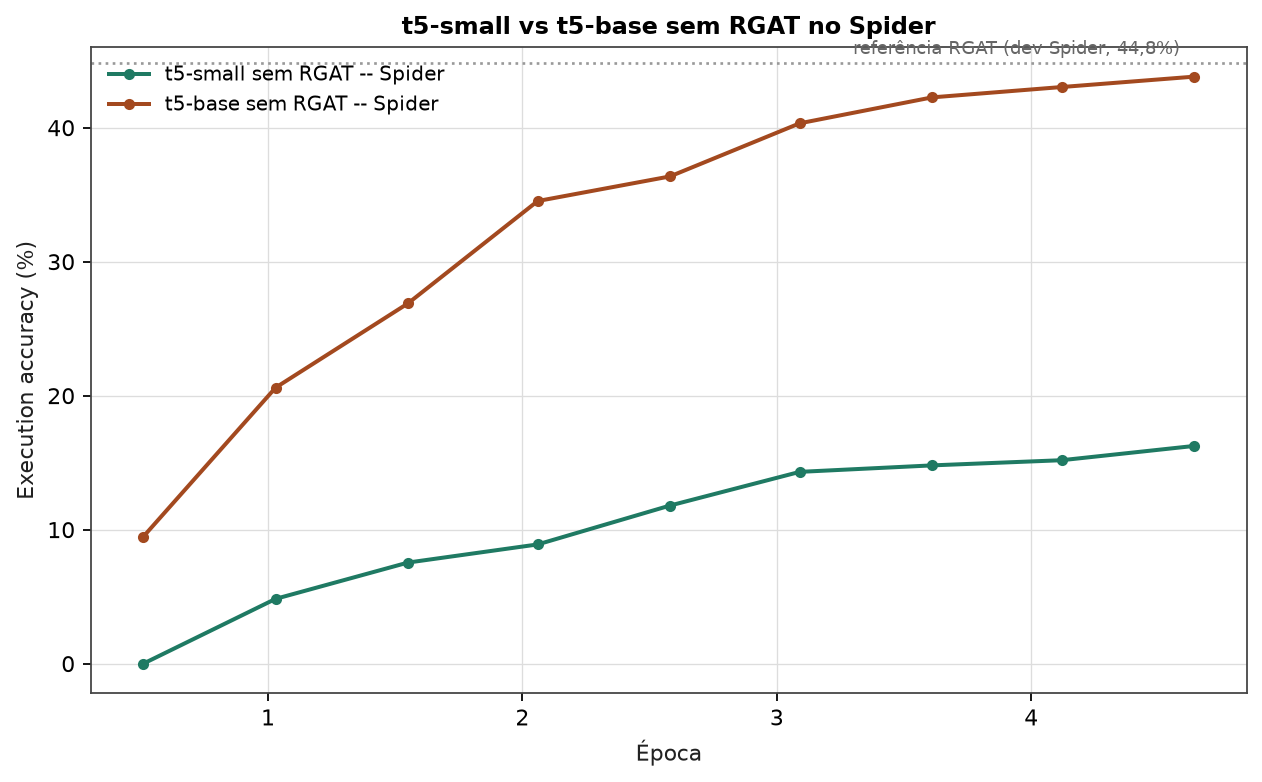
\includegraphics[width=0.95\textwidth]{spider_ablation_comparison.png}
\caption{Execution accuracy de validação ao longo do treino, t5-small vs.\ t5-base sem RGAT no Spider, com a referência RGAT marcada.}
\end{figure}

\begin{figure}[h]
\centering
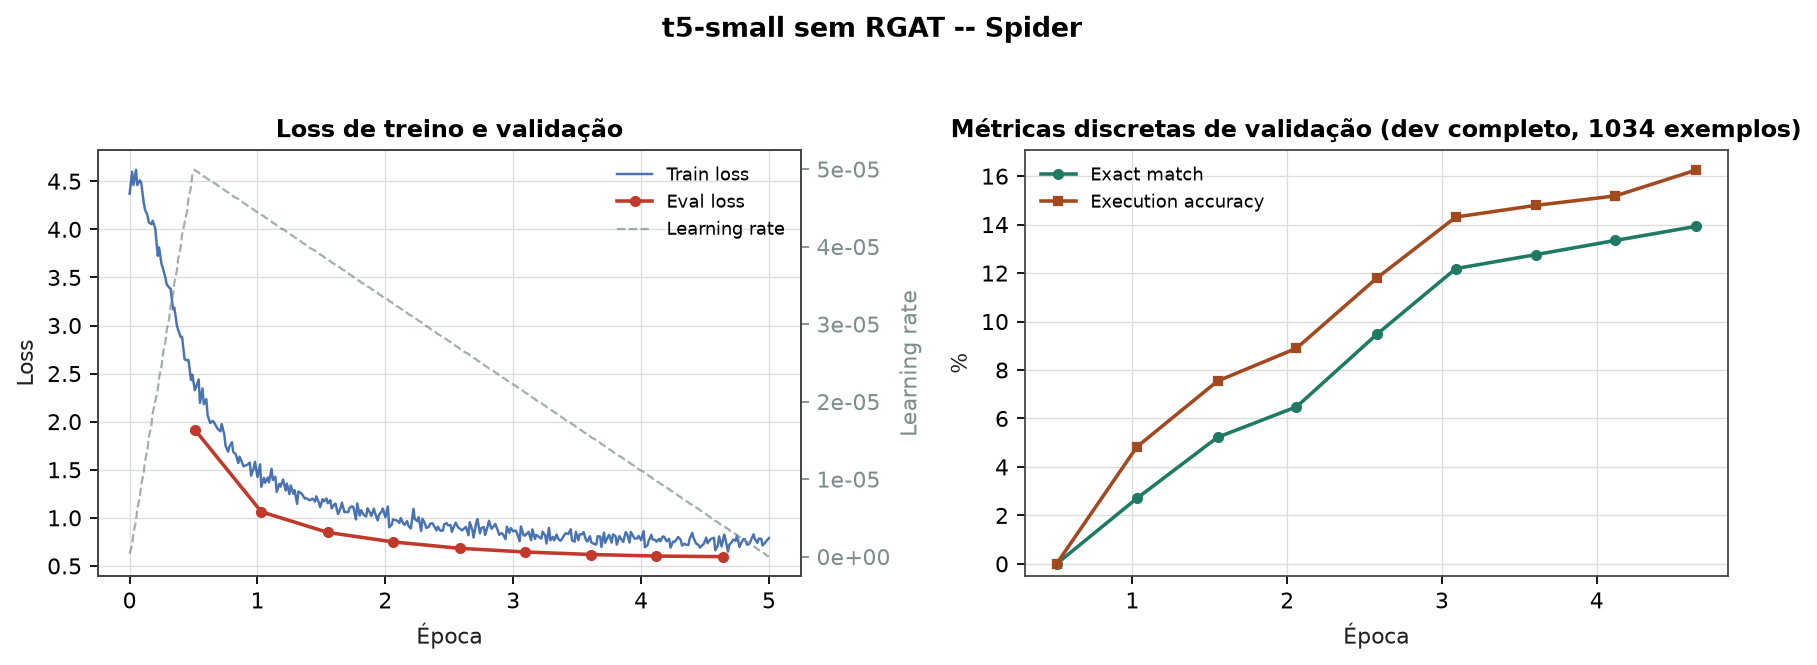
\includegraphics[width=0.95\textwidth]{spider_t5small_plain_training.png}
\caption{t5-small sem RGAT no Spider -- curvas de treino completas.}
\end{figure}

\begin{figure}[h]
\centering
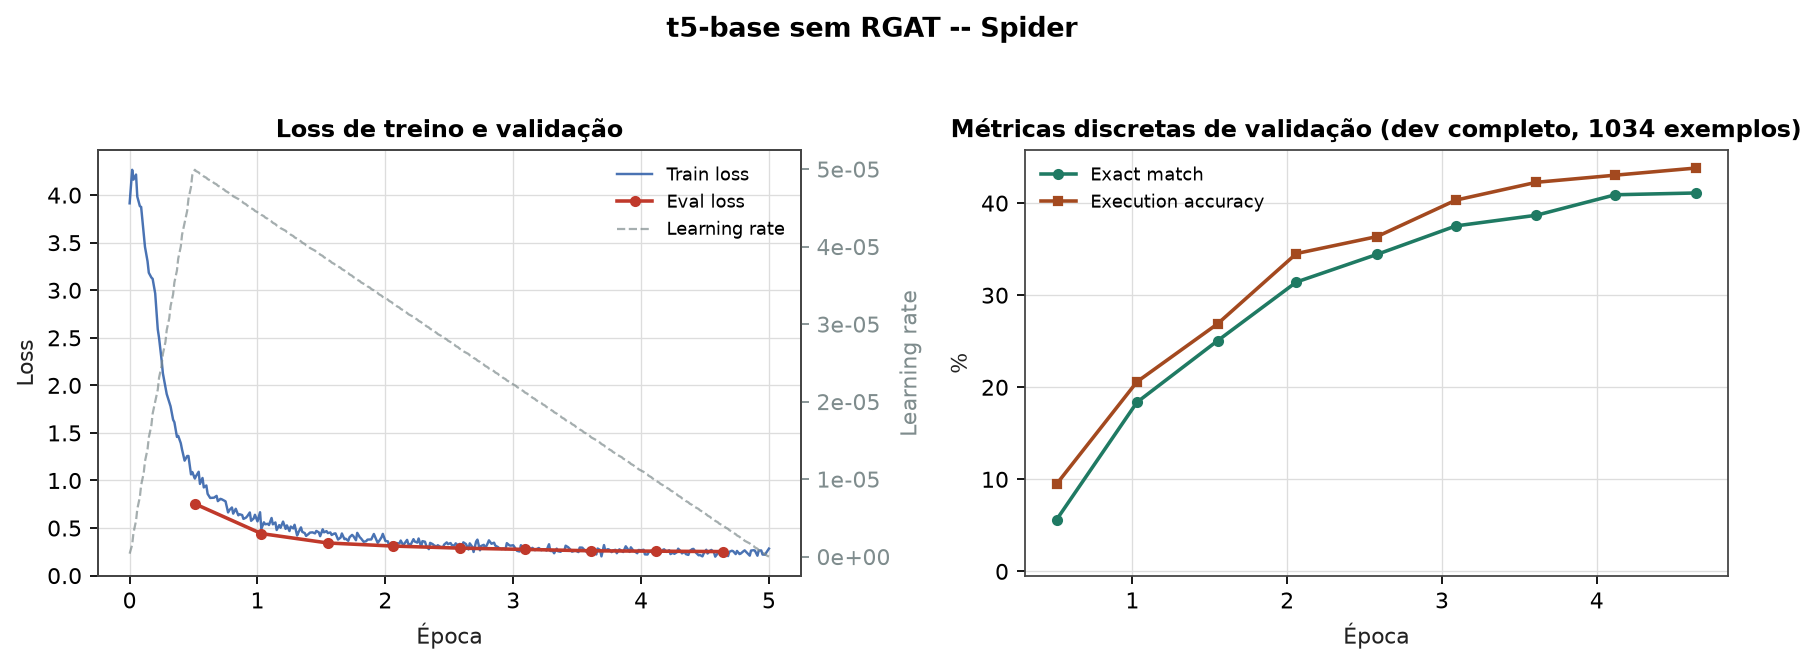
\includegraphics[width=0.95\textwidth]{spider_t5base_plain_training.png}
\caption{t5-base sem RGAT no Spider -- curvas de treino completas.}
\end{figure}

\end{document}
